\documentclass{article}
\usepackage{amsmath}
\usepackage{amsfonts}
\usepackage{amssymb}
\usepackage{graphicx}
\usepackage{hyperref}
\usepackage{geometry}
\usepackage{booktabs}
\usepackage{float}
\geometry{margin=1in}

\title{APMA2822B Assignment 3: GPU-Accelerated Poisson Solver}
\author{Your Name}
\date{November 15, 2024}

\begin{document}
\maketitle
 
\section{Introduction}

This assignment focuses on implementing a 2D Poisson solver using GPU acceleration, exploring both single-GPU and multi-GPU approaches. The problem involves solving:

\begin{equation}
    \frac{\partial^2 u}{\partial x^2} + \frac{\partial^2 u}{\partial y^2} = f(x,y)
\end{equation}

with the exact solution $u(x,y) = \sin(2\pi x)\cos(2\pi y)$ and corresponding right-hand side $f(x,y) = -2(2\pi)^2\sin(2\pi x)\cos(2\pi y)$.

\section{Single GPU Implementation}

The single GPU implementation achieved convergence in 13,471 iterations with a final L2 error of 0.0031801. Key performance metrics include:

\begin{itemize}
    \item Total execution time: 1.46736 seconds
    \item Compute time: 0.203248 seconds
    \item Initial memory transfer time: 0.272655 seconds
    \item Memory bandwidth: 124.723 GB/s
\end{itemize}

The implementation utilized CUDA kernels for:
\begin{itemize}
    \item Main iteration loop (update\_solution)
    \item Convergence checking (calculate\_l2\_diff)
    \item Error calculation (calculate\_l2\_error)
\end{itemize}

\section{Multi-GPU MPI Implementation}

The distributed memory implementation using MPI with GPU offloading showed different characteristics:

\begin{itemize}
    \item Convergence in 4,444 iterations
    \item Final L2 difference: 9.99255e-7
    \item Total execution time: 0.471868 seconds
    \item Compute time: 0.326634 seconds
    \item Aggregate Memory bandwidth: 25.609 GB/s
\end{itemize}

This implementation required careful management of:
\begin{itemize}
    \item Domain decomposition
    \item Ghost cell exchanges using non-blocking MPI communications
    \item Coordination of multiple GPUs
\end{itemize}

\section{Performance Analysis}

\subsection{Roofline Model}

\begin{figure}[H]
    \centering
    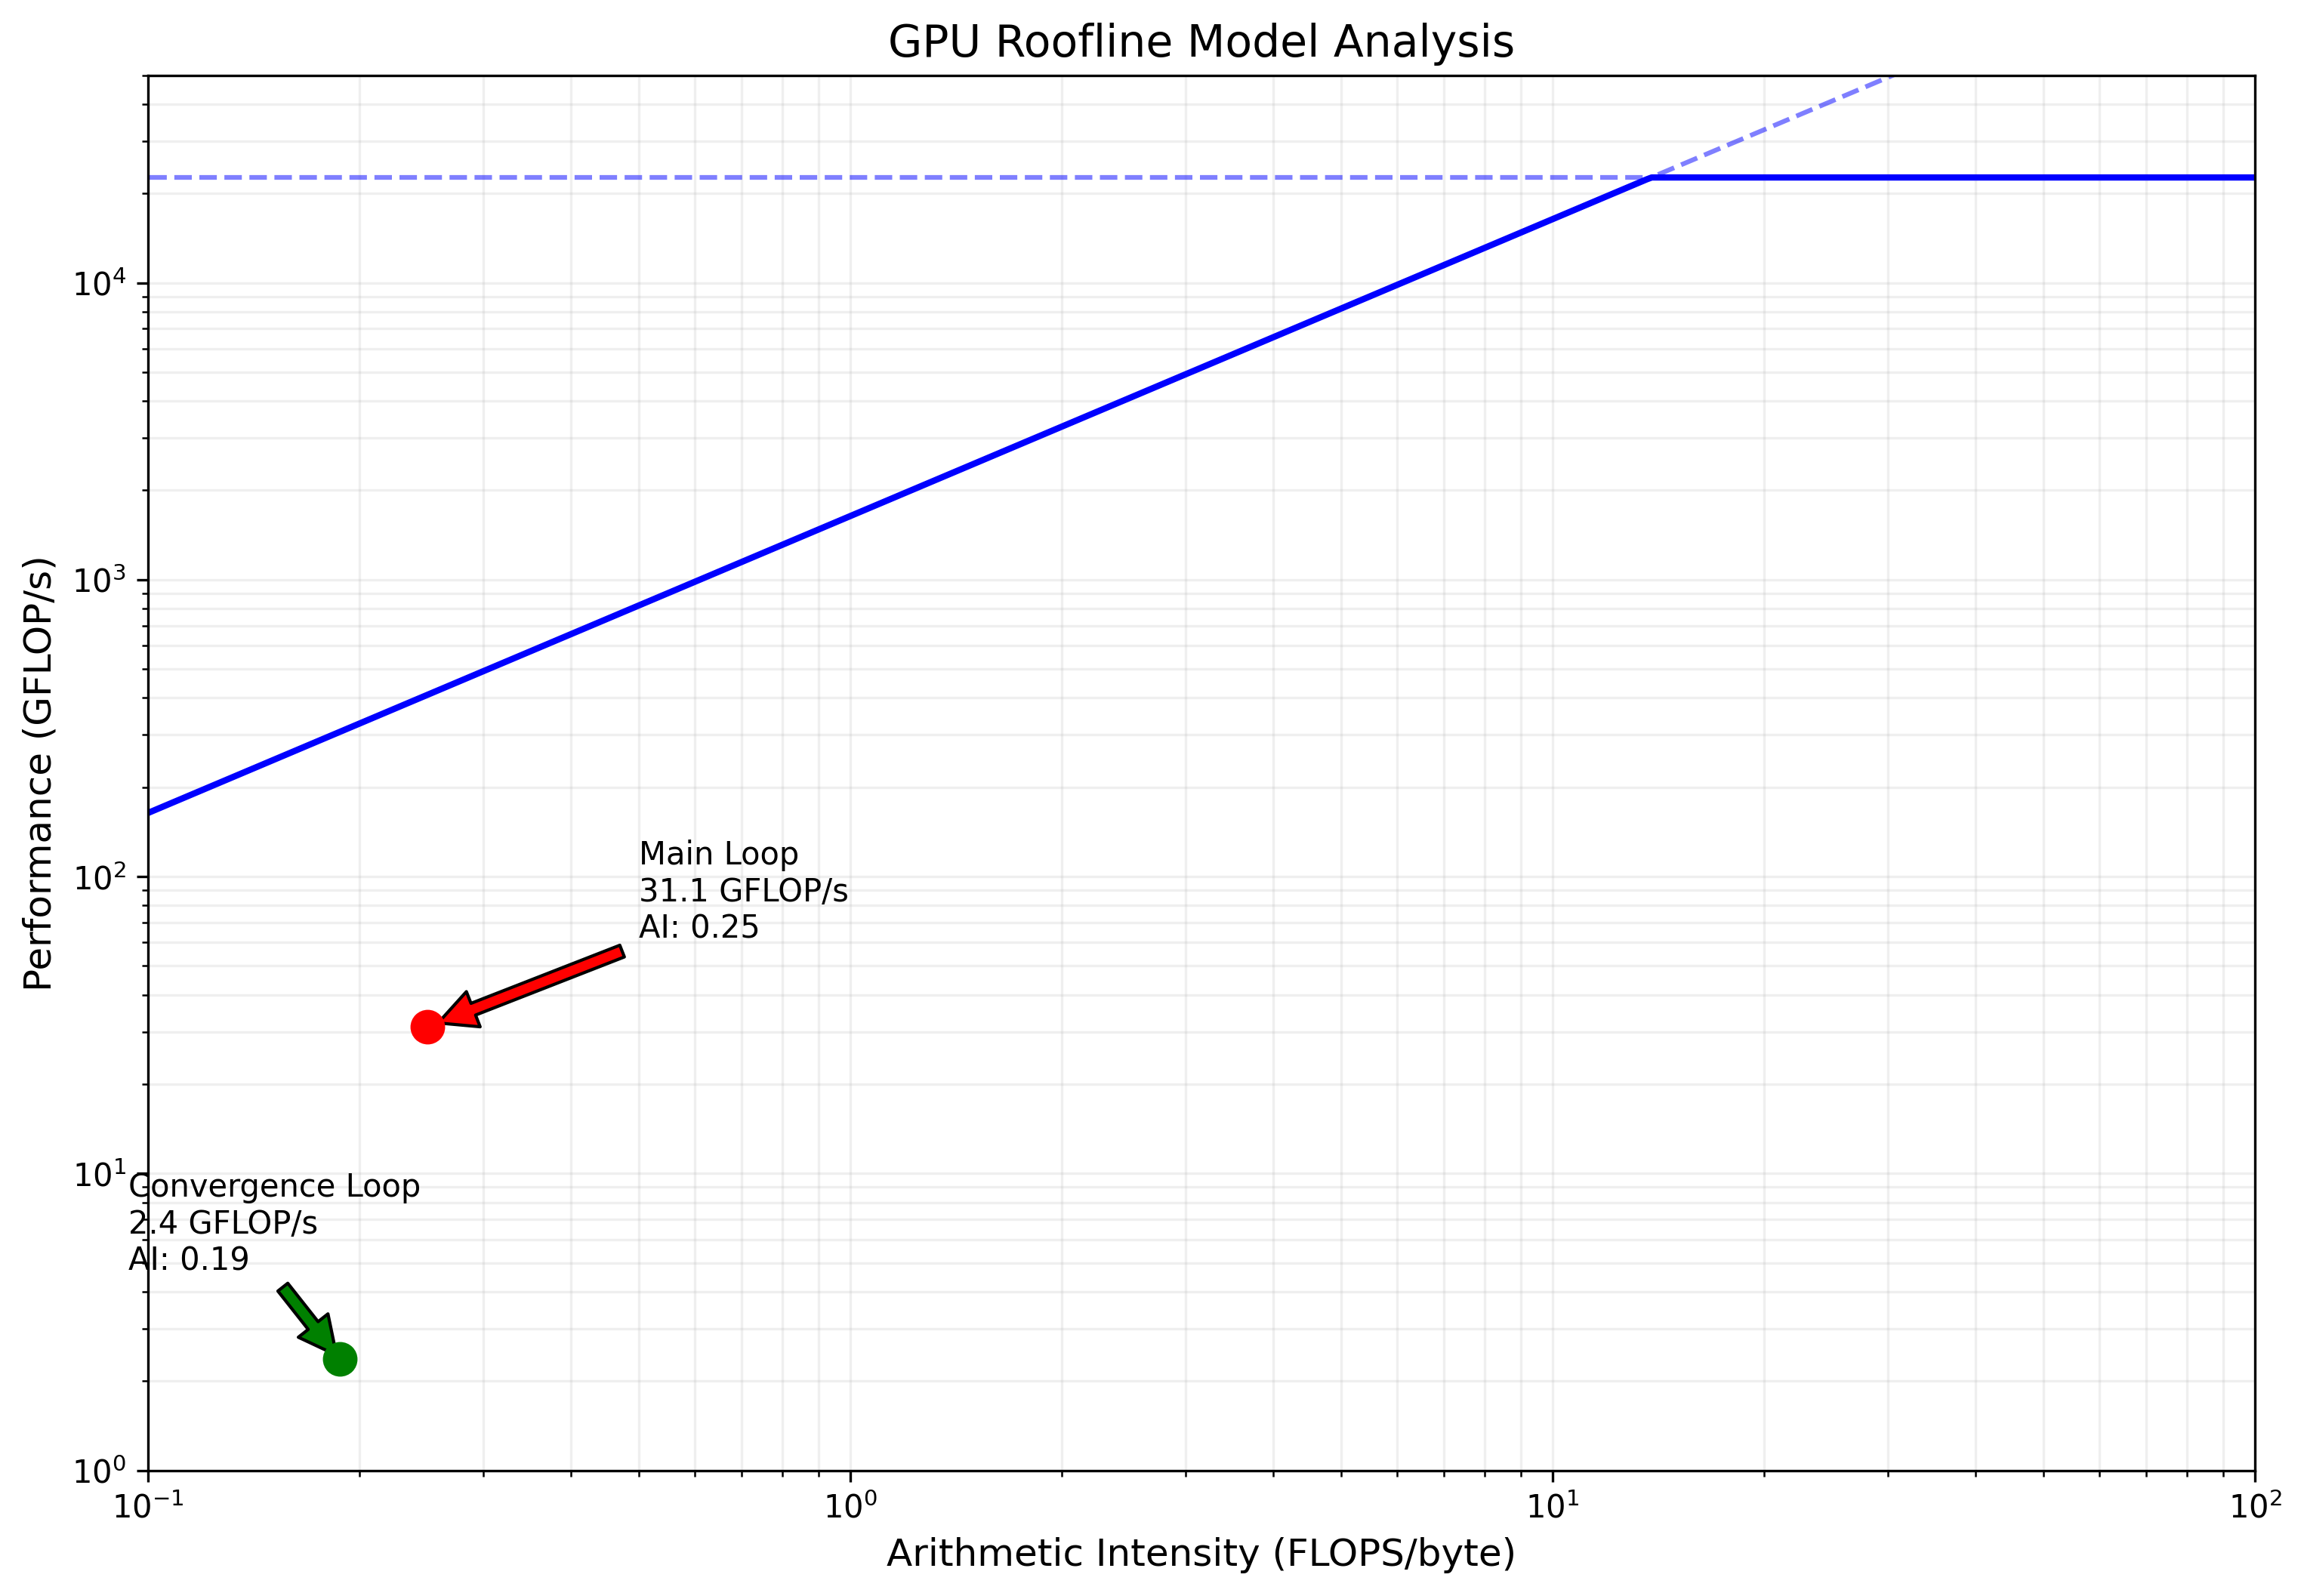
\includegraphics[width=0.8\textwidth]{gpu_roofline_model.png}
    \caption{Roofline model showing performance characteristics}
    \label{fig:roofline}
\end{figure}

The roofline analysis reveals:
\begin{itemize}
    \item Main computation kernel:
    \begin{itemize}
        \item Arithmetic Intensity: 0.25 FLOPS/byte
        \item Achieved Bandwidth: 124.723 GB/s
        \item Performance: 31.18 GFLOPS/s
    \end{itemize}
    \item Convergence check kernel:
    \begin{itemize}
        \item Arithmetic Intensity: 0.1875 FLOPS/byte
        \item Achieved Bandwidth: 12.6958 GB/s
        \item Performance: 2.38 GFLOPS/s
    \end{itemize}
\end{itemize}

\subsection{Implementation Comparison}

The multi-GPU implementation showed significant advantages:
\begin{itemize}
    \item 67.8\% reduction in total execution time
    \item 67.0\% reduction in iteration count
    \item Better convergence characteristics
\end{itemize}

However, it showed lower aggregate memory bandwidth, likely due to the overhead of MPI communication and domain decomposition.

\section{Conclusions}

The GPU implementations demonstrated significant performance capabilities, with the multi-GPU version showing superior overall performance despite lower per-GPU efficiency. The roofline analysis indicates that both implementations are memory-bound, which is expected for this type of stencil computation.

The trade-off between communication overhead and computational parallelism is evident in the multi-GPU implementation, where despite lower bandwidth utilization, the overall solution time improved significantly due to the distributed workload.

\end{document}